% =====================================================================
%  CARA DRIVER COMPANION DC-1 — FULL USER MANUAL
%  Course : Electronic Product Development (Sessional) — Lab, Group 7
%  Follows: IEC/IEEE 82079-1 (preparation of instructions for use),
%           ISO/IEC/IEEE 26514 (information for users),
%           ANSI Z535.6 / ISO 3864 signal words (DANGER / WARNING /
%           CAUTION / NOTICE), ISO 7010 and IEC 60417 / ISO 7000 symbols,
%           IEC 62368-1 (instructional safeguards), IEC 60529 (IP code).
%
%  BEFORE PRINTING
%  1. Fill in the FILL-IN FIELDS below (website, e-mail). Empty fields
%     print a marked gap, so nothing is invented.
%  2. Put the photos in photos/ with the names in PHOTO_SHOT_LIST.md.
%     A missing photo prints a dashed frame with its file name.
%  3. Compile: pdflatex; makeindex -s cara-index.ist <file>.idx; pdflatex; pdflatex.
% =====================================================================
\documentclass[11pt,a4paper,oneside]{report}
\usepackage[a4paper,margin=1in,headheight=14pt]{geometry}
\usepackage[T1]{fontenc}
\usepackage{helvet}
\usepackage{times}
\usepackage{amsmath,amssymb}
\usepackage{graphicx}
\usepackage{booktabs,array,longtable,tabularx,multirow}
\usepackage[table]{xcolor}
\usepackage{enumitem}
\usepackage{fancyhdr}
\usepackage{caption}
\usepackage{float}
\usepackage{lastpage}
\usepackage{makeidx}
\usepackage{etoolbox}
\usepackage{tikz}
\usetikzlibrary{arrows.meta,shapes.geometric,positioning,calc,fit}
\usepackage[most]{tcolorbox}
\usepackage{titlesec}
\usepackage{qrcode}
\usepackage[colorlinks=true,linkcolor=NavyBlue,urlcolor=NavyBlue]{hyperref}
\setlength{\emergencystretch}{3em}
\makeindex
% Index look: letter headings in the house style, page numbers set right.
\newcommand{\idxhead}[1]{\par\vspace{8pt}{\sffamily\bfseries\large\color{NavyBlue}#1}\par\nopagebreak\vspace{2pt}{\color{NavyBlue!40}\hrule height 0.6pt}\nopagebreak\vspace{3pt}}
\renewcommand{\indexspace}{}
\newcommand{\idxpage}[1]{#1}

\definecolor{NavyBlue}{RGB}{31,56,100}
\definecolor{LightBlue}{RGB}{220,230,241}
\definecolor{WarnYellow}{RGB}{255,204,0}
\definecolor{Amber}{RGB}{242,179,61}
\newcommand{\hdr}[1]{\cellcolor{LightBlue}\textbf{#1}}
\newcommand{\menu}[1]{\textsf{\textbf{#1}}}
\newcommand{\ui}[1]{\textsf{#1}}
\newcommand{\say}[1]{``\textit{#1}''}

% ---------- FILL-IN FIELDS (leave empty until you have them) ----------
\newcommand{\Website}{https://ahmed12-stack.github.io/driver-companion_EPD/}  % product website (GitHub Pages)
\newcommand{\SupportMail}{cara.support.dc1@gmail.com}  % support e-mail

% ---------- DOCUMENT FIELDS ----------
\newcommand{\Brand}{CARA}
\newcommand{\AppName}{Driver Companion} % the app's name on the phone
\newcommand{\ProductName}{CARA Driver Companion}
\newcommand{\ModelNo}{DC-1}
\newcommand{\InstituteName}{KIIT Deemed to be University}
\newcommand{\DeptName}{School of Electronics Engineering}
\newcommand{\TeamName}{EPD Group 7}
\newcommand{\DocNo}{EPD/UM/2024-28/G07}
\newcommand{\DocRev}{1.0}
\newcommand{\IssueDate}{06-11-2026}
\newcommand{\FWVer}{0.2.0}
\newcommand{\AppVer}{0.3.0}

% ---------- HELPERS ----------
\newcommand{\field}[2]{\ifdefempty{#1}{\textcolor{NavyBlue!70}{[#2 --- to be added]}}{\expandafter\nolinkurl\expandafter{#1}}}
\newcommand{\photo}[4]{\IfFileExists{photos/#1}%
 {\includegraphics[width=#2,height=#3,keepaspectratio]{photos/#1}}%
 {\tikz\node[draw=NavyBlue!60,dashed,fill=LightBlue!35,minimum width=#2,minimum height=#3,align=center,
   font=\small\sffamily\color{NavyBlue}]{\textbf{PHOTO}\\#4\\[2pt]\texttt{\scriptsize photos/\detokenize{#1}}};}}
% A phone screenshot in a simple phone frame.
\newcommand{\screen}[2]{\begin{tikzpicture}
 \node[inner sep=0] (s) {\photo{#1}{3.6cm}{7.4cm}{#2}};
 \draw[black!75,line width=2.2pt,rounded corners=7pt] ($(s.south west)+(-0.12,-0.3)$) rectangle ($(s.north east)+(0.12,0.3)$);
 \end{tikzpicture}}

% ---------- CHAPTER / HEADER STYLE ----------
\titleformat{\chapter}[display]{\bfseries\Huge\color{NavyBlue}\sffamily}{\filleft\Large\chaptertitlename\ \thechapter}{8pt}{\titlerule[1.2pt]\vspace{6pt}}
\titlespacing*{\chapter}{0pt}{-10pt}{24pt}
\titleformat{\section}{\Large\bfseries\color{NavyBlue}\sffamily}{\thesection}{0.6em}{}
\titleformat{\subsection}{\large\bfseries\color{NavyBlue}\sffamily}{\thesubsection}{0.6em}{}
\pagestyle{fancy}\fancyhf{}
\fancyhead[L]{\small\sffamily \ProductName\ \ModelNo\ User Manual}
\fancyhead[R]{\small\sffamily \DocNo\ Rev \DocRev}
\fancyfoot[C]{\small\sffamily Page \thepage\ of \pageref{LastPage}}
\renewcommand{\headrulewidth}{0.4pt}
\fancypagestyle{plain}{\fancyhf{}\fancyfoot[C]{\small\sffamily Page \thepage\ of \pageref{LastPage}}\renewcommand{\headrulewidth}{0pt}}

% ---------- SYMBOLS ----------
\newcommand{\warnsym}[1][0.55cm]{\begin{tikzpicture}[baseline=-0.1ex]
 \fill[WarnYellow,draw=black,line width=0.6pt,rounded corners=1pt] (0,0)--(#1,0)--(#1/2,#1*0.87)--cycle;
 \node[font=\bfseries\scriptsize] at (#1/2,#1*0.3) {!};\end{tikzpicture}}
\newcommand{\elecsym}[1][0.55cm]{\begin{tikzpicture}[baseline=-0.1ex]
 \fill[WarnYellow,draw=black,line width=0.6pt,rounded corners=1pt] (0,0)--(#1,0)--(#1/2,#1*0.87)--cycle;
 \fill[black] (#1*0.55,#1*0.68)--(#1*0.33,#1*0.34)--(#1*0.48,#1*0.34)--(#1*0.40,#1*0.12)--(#1*0.68,#1*0.45)--(#1*0.52,#1*0.45)--cycle;
 \end{tikzpicture}}
\newcommand{\hotsym}[1][0.55cm]{\begin{tikzpicture}[baseline=-0.1ex]
 \fill[WarnYellow,draw=black,line width=0.6pt,rounded corners=1pt] (0,0)--(#1,0)--(#1/2,#1*0.87)--cycle;
 \foreach \x in {0.36,0.5,0.64}{\draw[line width=0.5pt] (#1*\x,#1*0.15) .. controls (#1*\x+0.04,#1*0.3) and (#1*\x-0.04,#1*0.4) .. (#1*\x,#1*0.55);}
 \end{tikzpicture}}
\newcommand{\mandsym}[1][0.5cm]{\begin{tikzpicture}[baseline=-0.5ex]
 \fill[blue!70!black] (0,0) circle (#1/2);\node[white,font=\bfseries\small] at (0,0) {i};\end{tikzpicture}}
\newcommand{\prohibsym}[1][0.5cm]{\begin{tikzpicture}[baseline=-0.5ex]
 \draw[red!80!black,line width=1.4pt,fill=white] (0,0) circle (#1/2);\draw[red!80!black,line width=1.4pt] (-#1*0.35,#1*0.35)--(#1*0.35,-#1*0.35);\end{tikzpicture}}
\newcommand{\phonesym}[1][0.5cm]{\begin{tikzpicture}[baseline=-0.5ex]
 \draw[red!80!black,line width=1.3pt,fill=white] (0,0) circle (#1/2);
 \draw[rounded corners=0.8pt,line width=0.6pt] (-#1*0.13,-#1*0.24) rectangle (#1*0.13,#1*0.24);
 \draw[red!80!black,line width=1.3pt] (-#1*0.35,#1*0.35)--(#1*0.35,-#1*0.35);\end{tikzpicture}}
\newcommand{\weeesym}[1][0.5cm]{\begin{tikzpicture}[baseline=0pt,scale=#1/0.5cm]
 \draw[line width=0.6pt] (0.1,0.05) rectangle (0.4,0.32);\draw[line width=0.6pt] (0.05,0.32)--(0.45,0.32);
 \draw[line width=0.6pt] (0.2,0.32) arc(180:0:0.05);
 \draw[line width=0.8pt,red] (0,0)--(0.5,0.5);\draw[line width=0.8pt,red] (0,0.5)--(0.5,0);
 \fill (0,-0.12) rectangle (0.5,-0.04);\end{tikzpicture}}
\newcommand{\dcsym}{\tikz[baseline=-0.5ex]{\draw[line width=0.8pt] (0,0.06)--(0.45,0.06);\draw[line width=0.8pt,dash pattern=on 1.5pt off 1.5pt] (0,-0.06)--(0.45,-0.06);}}
\newcommand{\indoorsym}{\tikz[baseline=-0.6ex]{\draw[line width=0.7pt] (0,-0.15)--(0,0.12)--(0.22,0.28)--(0.44,0.12)--(0.44,-0.15)--cycle;\fill (0.16,-0.15) rectangle (0.28,0.02);}}
\newcommand{\callout}[1]{\tikz[baseline=-0.6ex]\node[circle,draw=NavyBlue,fill=white,text=NavyBlue,inner sep=1pt,font=\bfseries\scriptsize]{#1};}
\newcommand{\sdot}[1]{\tikz[baseline=-0.5ex]\fill[#1,draw=black!50,line width=0.3pt] (0,0) circle (0.1cm);}
\newcommand{\spk}{\tikz[baseline=-0.5ex]{\fill[NavyBlue] (0,-0.07) rectangle (0.08,0.07);\fill[NavyBlue] (0.08,-0.07)--(0.18,-0.15)--(0.18,0.15)--(0.08,0.07)--cycle;
 \draw[NavyBlue,line width=0.6pt] (0.24,-0.08) arc(-40:40:0.12);\draw[NavyBlue,line width=0.6pt] (0.29,-0.13) arc(-40:40:0.2);}}

% ---------- SIGNAL-WORD BOXES (ANSI Z535.6 / ISO 3864) ----------
\newtcolorbox{danger}{enhanced,colback=red!6,colframe=red!75!black,boxrule=1pt,arc=2pt,left=4pt,right=4pt,top=3pt,bottom=3pt,
  title={\elecsym\ \ DANGER},fonttitle=\bfseries\sffamily,coltitle=white,colbacktitle=red!75!black}
\newtcolorbox{warning}{enhanced,colback=orange!8,colframe=orange!85!black,boxrule=1pt,arc=2pt,left=4pt,right=4pt,top=3pt,bottom=3pt,
  title={\warnsym\ \ WARNING},fonttitle=\bfseries\sffamily,coltitle=black,colbacktitle=orange!85!black}
\newtcolorbox{caution}{enhanced,colback=yellow!10,colframe=yellow!60!black,boxrule=1pt,arc=2pt,left=4pt,right=4pt,top=3pt,bottom=3pt,
  title={\warnsym\ \ CAUTION},fonttitle=\bfseries\sffamily,coltitle=black,colbacktitle=WarnYellow}
\newtcolorbox{notice}{enhanced,colback=blue!5,colframe=blue!60!black,boxrule=1pt,arc=2pt,left=4pt,right=4pt,top=3pt,bottom=3pt,
  title={NOTICE},fonttitle=\bfseries\sffamily,coltitle=white,colbacktitle=blue!60!black}
\newtcolorbox{tip}{enhanced,colback=green!5,colframe=green!45!black,boxrule=0.8pt,arc=2pt,left=4pt,right=4pt,top=2pt,bottom=2pt,
  title={\mandsym[0.38cm]\ \ TIP},fonttitle=\bfseries\sffamily,coltitle=white,colbacktitle=green!45!black}

\begin{document}
\pagenumbering{roman}

% =====================================================================
%  TITLE PAGE
% =====================================================================
\begin{titlepage}
\sffamily\begin{center}
{\large \InstituteName\\ \DeptName}\\[1.0cm]
\photo{um_title.jpg}{10cm}{6.2cm}{The \Brand\ \ModelNo\ unit on a dashboard}\\[0.9cm]
{\Huge\bfseries\color{NavyBlue} \ProductName}\\[0.3cm]
{\Large Model \ModelNo}\\[0.8cm]
\rule{0.7\linewidth}{0.8pt}\\[0.5cm]
{\Huge\bfseries USER MANUAL}\\[0.4cm]
{\large Installation \textbullet\ Operation \textbullet\ Maintenance \textbullet\ Disposal}\\[0.5cm]
\rule{0.7\linewidth}{0.8pt}
\vfill
\renewcommand{\arraystretch}{1.3}
\begin{tabular}{rl}
Document no.: & \DocNo\\ Revision: & \DocRev\\ Applies to device software: & \FWVer\ and later\\ Applies to app: & \AppVer\ and later\\ Date of issue: & \IssueDate\\
\end{tabular}\\[0.6cm]
{\small\warnsym\ \ \textbf{Read this manual, especially Chapter~\ref{ch:safety}, before using the product. Keep it for future reference.}}
\end{center}
\end{titlepage}

% =====================================================================
%  NOTICES, REVISION HISTORY
% =====================================================================
\chapter*{Notices and Document Information}
\addcontentsline{toc}{chapter}{Notices and Document Information}
\section*{Copyright and Disclaimer}
\copyright\ 2026 \TeamName, \DeptName, \InstituteName. All rights reserved. No part of this manual may be reproduced without written permission. The information in this manual is subject to change without notice.

\ProductName\ was developed as a course project in \emph{Electronic Product Development (Sessional)}. It is an \textbf{educational prototype}: it has not been certified for commercial sale, and it is a driver aid only. It does not drive, brake or steer the vehicle, and it does not replace the driver's own attention to the road and the road signs.

\textbf{Trademarks.} Raspberry Pi is a trademark of Raspberry Pi Ltd. Android is a trademark of Google LLC. The Bluetooth word mark is owned by Bluetooth SIG, Inc. WhatsApp, Instagram and Messenger are trademarks of Meta Platforms, Inc.; Telegram, Signal and Gmail belong to their owners. Their use here does not mean that these owners endorse this product.

\section*{Revision History}
\begin{table}[H]\centering\small
\begin{tabular}{|c|c|p{0.42\linewidth}|>{\raggedright\arraybackslash}p{0.24\linewidth}|}\hline
\hdr{Rev.} & \hdr{Date} & \hdr{Change} & \hdr{Applies to}\\ \hline
1.0 & \IssueDate & First release, with the \ModelNo\ prototype & Device software \FWVer; app \AppVer\\ \hline
\end{tabular}\end{table}

\section*{Related Documents}
\begin{table}[H]\centering\small
\begin{tabular}{|l|l|}\hline
\hdr{Document} & \hdr{Number}\\ \hline
Quick Start Guide (one page) & EPD/QSG/2024-28/G07\\ \hline
Product Design Report & EPD/PDR/2024-28/G07\\ \hline
Product Test Report & EPD/PTR/2024-28/G07\\ \hline
\end{tabular}\end{table}

\section*{Open-Source Components}
The product runs open-source software. Each component stays under its own licence; the licence texts are available on request from the support contact in Chapter~\ref{ch:compliance}.
\begin{table}[H]\centering\small
\begin{tabularx}{\linewidth}{|l|X|l|}\hline
\hdr{Component} & \hdr{Used for} & \hdr{Licence}\\ \hline
Raspberry Pi OS, Linux, BlueZ & Operating system and Bluetooth & GPL-2.0 and others\\ \hline
Eclipse Mosquitto & Internal message board between modules & EPL-2.0 / EDL-1.0\\ \hline
LiteRT (TensorFlow Lite) & Running the road-sign model & Apache-2.0\\ \hline
Piper; voice \emph{en\_GB-cori-medium} & Natural speech & MIT; see voice model card\\ \hline
eSpeak NG & Back-up speech & GPL-3.0\\ \hline
llama.cpp; Qwen2.5-0.5B-Instruct & On-device trip remark & MIT; Apache-2.0\\ \hline
osmdroid; OpenStreetMap data & Trip map in the app & Apache-2.0; ODbL\\ \hline
IBM Plex Sans and Mono & App fonts & SIL OFL 1.1\\ \hline
\end{tabularx}\end{table}

\clearpage
\tableofcontents
\clearpage
\listoffigures
\clearpage
\listoftables
\clearpage
\pagenumbering{arabic}

% =====================================================================
\chapter*{About This Manual}
\addcontentsline{toc}{chapter}{About This Manual}
\section*{Who Should Read It}
This manual is written for \textbf{drivers} who use \ProductName\ in a car, and for the person who sets it up for them. No electronics knowledge is needed. Sections marked \emph{Technician only} are for trained service staff.

\section*{How the Manual Is Organised}
\begin{table}[H]\centering\small
\begin{tabularx}{\linewidth}{|l|X|}\hline
\hdr{Chapter} & \hdr{Use it when you want to \ldots}\\ \hline
1~Safety Information & \ldots use the product without harm to people or property\\ \hline
2~Product Overview & \ldots learn what is in the box, the parts, the app and the specifications\\ \hline
3~Installation and Setup & \ldots power, place and pair the product for the first time\\ \hline
4~Operation & \ldots use the product on every drive\\ \hline
5~Maintenance & \ldots clean, update or service the product\\ \hline
6~Troubleshooting & \ldots find the cause of a problem and fix it\\ \hline
7~Disposal and Environment & \ldots recycle or dispose of the product\\ \hline
8~Warranty, Support, Compliance & \ldots get help or check the product's status\\ \hline
\end{tabularx}\end{table}

\section*{Conventions Used}
\begin{table}[H]\centering\small
\begin{tabularx}{\linewidth}{|c|l|X|}\hline
\hdr{Symbol} & \hdr{Signal word} & \hdr{Meaning}\\ \hline
\elecsym & \textbf{DANGER} & Hazard that \emph{will} cause death or serious injury if not avoided.\\ \hline
\warnsym & \textbf{WARNING} & Hazard that \emph{can} cause death or serious injury if not avoided.\\ \hline
\warnsym & \textbf{CAUTION} & Hazard that can cause minor or moderate injury.\\ \hline
--- & \textbf{NOTICE} & Risk of damage to the product or data; no personal injury.\\ \hline
\mandsym & \textbf{TIP / NOTE} & Useful information for better results.\\ \hline
\ui{Pair} & Sans-serif text & Names of buttons and screen text in the app.\\ \hline
\spk\ \say{Text} & Quoted italics & Words the unit speaks.\\ \hline
1., 2., 3.\ & Numbered steps & Do the steps in the given order.\\ \hline
\callout{1} & Callout number & Refers to a numbered part in Figure~\ref{fig:parts}.\\ \hline
\end{tabularx}\end{table}

% =====================================================================
\chapter{Safety Information}\label{ch:safety}\index{safety}\index{warnings|see{safety}}

\section{Intended Use}\index{intended use}\index{misuse}\index{driver aid}
\ProductName\ is a driver aid for private cars. A camera reads road signs ahead and the unit speaks them aloud; it warns when the car is over the last speed limit read; it announces chosen phone messages and calls; and it speaks a short summary at the end of each drive. It is used inside the passenger compartment by adult drivers, together with an Android phone. Use it only as described in this manual.

\begin{warning}
Do not rely on the product to drive safely. It can miss a sign, read a sign wrongly, or stay silent (for example in rain, at night, in glare or when the camera is blocked). The road signs, traffic rules and the traffic around you always come first. Do not use the product as a speed limiter, for professional or commercial driving, for vehicles other than cars, or for any safety-critical purpose. Misuse can cause accidents and voids the warranty.
\end{warning}

\section{Driving Safety}\index{driving safety}\index{distraction}\index{airbag}\index{phone!while driving}\index{volume!safe level}
\begin{warning}
\textbf{Distraction can cause a crash.} Set up the app, the volume and the announced apps \emph{before} you start driving. Do not hold, look at or operate the phone or the unit while the vehicle is moving. Using a hand-held phone while driving is an offence in India and in many other countries.
\end{warning}
\begin{itemize}[leftmargin=*]
\item Place the unit so that it does not block your view of the road, the mirrors or the instruments (Section~\ref{sec:place}).
\item Never place the unit on or in front of an airbag cover. An airbag can throw it at high speed.
\item Make sure the unit, its power cable and the button leads cannot slide, fall or get caught in the pedals or the steering wheel during braking or turning.
\item Keep the volume loud enough to hear alerts, but not so loud that you cannot hear horns or emergency sirens.
\item If an alert is unclear, keep driving safely and look at the actual sign. Do not stop suddenly to check the unit.
\end{itemize}

\section{General Safety Instructions}\index{safety!general instructions}\index{children and pets}\index{damage, signs of}
\begin{itemize}[leftmargin=*]
\item Read all instructions before use and keep this manual with the product.
\item Use only the supplied cable and a power source that meets Section~\ref{sec:power}.
\item Do not use the product if it is damaged, has been dropped, smells of burning or shows signs of overheating.
\item Keep the product out of reach of small children and pets.
\item Do not modify the product or open the case; there are no user-serviceable parts inside.
\end{itemize}

\section{Electrical Safety}\index{electrical safety}\index{power source!requirements}\index{cable!damaged}
\begin{caution}
The product runs on low voltage (5\,V DC) only. Never connect it directly to the car's 12\,V wiring, to a mains socket, or to any adapter other than a USB power source. Do not use the product with wet hands, and keep drinks away from it.
\end{caution}
\begin{itemize}[leftmargin=*]
\item Use a USB power source rated 5\,V DC and at least 2.4\,A (power bank) or 2.5\,A (car charger).
\item Do not use the unit if its power cable is damaged; have the cable replaced by a technician.
\item Route the cable so it is not pinched by doors, seats or the glovebox.
\end{itemize}

\section{Power Bank Safety}\index{power bank!safety}\index{battery|see{power bank}}\index{lithium battery|see{power bank}}
\begin{warning}
The power bank (not supplied) contains a lithium battery. It can overheat, burst or catch fire if crushed, punctured, short-circuited or left in a hot car. Use a power bank with a recognised safety mark, do not leave it on the dashboard in the sun, and stop using it if it swells, leaks or gets hot.
\end{warning}

\section{Heat, Environment and Handling}\index{heat!hot surface}\index{parked car in the sun}\index{static electricity}\index{water and moisture}
\begin{caution}
\hotsym\ The case becomes warm during use. Do not cover the unit or wrap it in cloth, and do not put objects on the speaker \callout{2}.
\end{caution}
\begin{notice}
A parked car in the sun can reach 70\,\textdegree C or more. Do not leave the unit or the power bank in a parked car in direct sunlight. Keep the product away from water, dust and strong magnetic fields. Static electricity can damage the electronics; do not touch the port \callout{5} with bare metal.
\end{notice}

\section{Privacy and Data}\index{privacy}\index{data!stored in the unit}\index{camera!no images stored}\index{message text!privacy}\index{passengers}
\begin{notice}
The unit works without the internet. It does \emph{not} record video or store camera images. It keeps the last 20 trip summaries, with their routes, inside the unit and sends them only to your paired phone. Message and call text is spoken and then discarded; it is never saved in the unit. Only phones paired with the spoken code can connect. When you announce messages, other people in the car can hear them: switch \ui{Read message text} off or use \ui{Quiet mode} when you have passengers.
\end{notice}

\section{Symbols on the Product}\index{symbols on the product}\index{WEEE symbol}
\begin{table}[H]\centering\small
\caption{Symbols on the product and packaging}
\begin{tabularx}{\linewidth}{|c|X|l|}\hline
\hdr{Symbol} & \hdr{Meaning} & \hdr{Reference}\\ \hline
\mandsym & Read the user manual before use & ISO 7010 M002\\ \hline
\hotsym & Warning: hot surface & ISO 7010 W017\\ \hline
\weeesym & Separate collection of electrical and electronic equipment (do not put in household waste) & WEEE Directive 2012/19/EU\\ \hline
\dcsym & Direct current input & IEC 60417-5031\\ \hline
\indoorsym & For use inside the vehicle (indoor) only & IEC 60417-5957\\ \hline
\end{tabularx}\end{table}

% =====================================================================
\chapter{Product Overview}\label{ch:overview}
\section{Description and Key Features}\index{features}\index{road signs!overview}\index{overspeed!overview}\index{trip summary!overview}
\ProductName\ is a small dashboard unit that watches the road through a camera and \textbf{speaks} what the driver needs to know, so the driver's eyes stay on the road. It works with a free Android app. Key features:
\begin{itemize}[leftmargin=*]
\item \textbf{Road-sign alerts.} Reads 20 Indian road signs (IRC:67), such as speed limits, stop, school ahead and speed breaker, and speaks each one once, for example \say{Speed limit 50.}
\item \textbf{Overspeed warnings.} Compares the car's speed with the last speed limit read and says \say{Slow down. Speed limit 50.} when you are more than 5\,km/h over it.
\item \textbf{Phone announcements.} Reads out the sender of messages from apps you choose (for example WhatsApp), text messages and incoming calls, so you do not have to look at the phone.
\item \textbf{Trip summary.} When you park, it speaks a short summary of the drive, with one remark written by a small on-device AI. The trip, with its route on a map, appears in the app.
\item \textbf{Private by design.} Everything runs inside the unit, without the internet. No video is recorded.
\item \textbf{Natural voice.} A clear, natural female voice; three volume levels.
\end{itemize}

\section{What Is in the Box}\label{sec:box}\index{package contents}\index{box contents|see{package contents}}\index{what you also need}
\begin{table}[H]\centering\small
\caption{Package contents}
\begin{tabularx}{\linewidth}{|c|X|c|c|}\hline
\hdr{No.} & \hdr{Item} & \hdr{Qty} & \hdr{Check}\\ \hline
1 & \ProductName\ \ModelNo\ unit (camera and speaker built in) & 1 & $\square$\\ \hline
2 & USB power cable with USB-A plug (fitted to the unit) & 1 & $\square$\\ \hline
3 & Quick Start Guide & 1 & $\square$\\ \hline
4 & Full User Manual (this document) & 1 & $\square$\\ \hline
\end{tabularx}\end{table}
\textbf{You also need} (not supplied): an Android phone with Android 8.0 or newer, and a USB power bank of 5\,V, 2.4\,A or more (or a car USB charger, see Section~\ref{sec:power}). If any item is missing or damaged, contact support (Chapter~\ref{ch:compliance}) before using the product.

\section{Parts and Controls}\label{sec:parts}\index{parts and controls}\index{camera window}\index{speaker}\index{PAIR button}\index{TRIP button}\index{power cable}\index{button leads}\index{micro-USB|see{power cable}}\index{enclosure}

\begin{figure}[H]\centering
\begin{tabular}{@{}c@{\hspace{4mm}}c@{}}
\photo{parts_front.jpg}{0.49\linewidth}{6cm}{Front} & \photo{parts_back.jpg}{0.47\linewidth}{6cm}{Back}\\[2pt]
\small (a) Front: camera window and speaker & \small (b) Back: buttons and power cable\\
\end{tabular}
\caption{Parts and controls}\label{fig:parts}
\end{figure}

\begin{table}[H]\centering\small
\caption{Parts and controls (see Figure~\ref{fig:parts})}
\begin{tabularx}{\linewidth}{|c|l|X|}\hline
\hdr{No.} & \hdr{Part} & \hdr{Function}\\ \hline
\callout{1} & Camera window & Looks at the road ahead to read signs. Keep it clean and pointed forward\\ \hline
\callout{2} & Speaker & Speaks all alerts, announcements and summaries\\ \hline
\callout{3} & \ui{PAIR} button & Hold 5\,s to let a new phone pair (Section~\ref{sec:pair})\\ \hline
\callout{4} & \ui{TRIP} button & Press once before you set off (\say{Trip started.}), press again when you have parked (\say{Trip ended.})\\ \hline
\callout{5} & Power cable & USB cable with a USB-A plug, 5\,V DC. The unit switches on when the plug is connected to a power source\\ \hline
\end{tabularx}\end{table}
The \ui{PAIR} and \ui{TRIP} buttons hang on short leads at the back of the unit, so you can place them within reach of the driver's seat (Figure~\ref{fig:photos}). Both spring back when released. On this prototype the buttons carry the stickers \emph{WORK} (\ui{PAIR}) and \emph{TO DO} (\ui{TRIP}).

\begin{figure}[H]\centering
\photo{buttons_labeled.jpg}{0.72\linewidth}{6.5cm}{PAIR and TRIP buttons}
\caption{The \ui{PAIR} and \ui{TRIP} buttons and the power cable, at the back of the unit}\label{fig:photos}
\end{figure}

\section{The \AppName\ App}\label{sec:appoverview}\index{app!screens}\index{home screen}\index{trip details screen}\index{Announcements screen}
The app connects the phone to the unit over Bluetooth. It sends the phone's notifications and its GPS speed to the unit, lets you choose what is announced, and keeps every trip. It has three screens.
\begin{figure}[H]\centering
\begin{tabular}{ccc}
\screen{app_home.png}{Home screen} & \screen{app_trip.png}{Trip details} & \screen{app_settings.png}{Announcements}\\[2pt]
\small (a) Home & \small (b) Trip details & \small (c) Announcements\\
\end{tabular}
\caption{The \AppName\ app}\label{fig:app}
\end{figure}
\begin{itemize}[leftmargin=*]
\item \textbf{Home:} the connection status (a coloured dot and a word), the \ui{Phone GPS} line, the buttons \ui{Send test alert}, \ui{Disconnect} and \ui{Pair new}, and your three most recent trips.
\item \textbf{Trip details:} the route on a map, the distance, time and top speed, the spoken summary and the details of the drive.
\item \textbf{Announcements:} volume, message reading, quiet mode, calls, text messages and the apps to announce (Section~\ref{sec:settings}).
\end{itemize}

\section{System Block Diagram}\index{block diagram}
The following diagram shows how the parts of the product work together. It is provided for understanding only; it is not needed for normal use.
\begin{figure}[H]\centering
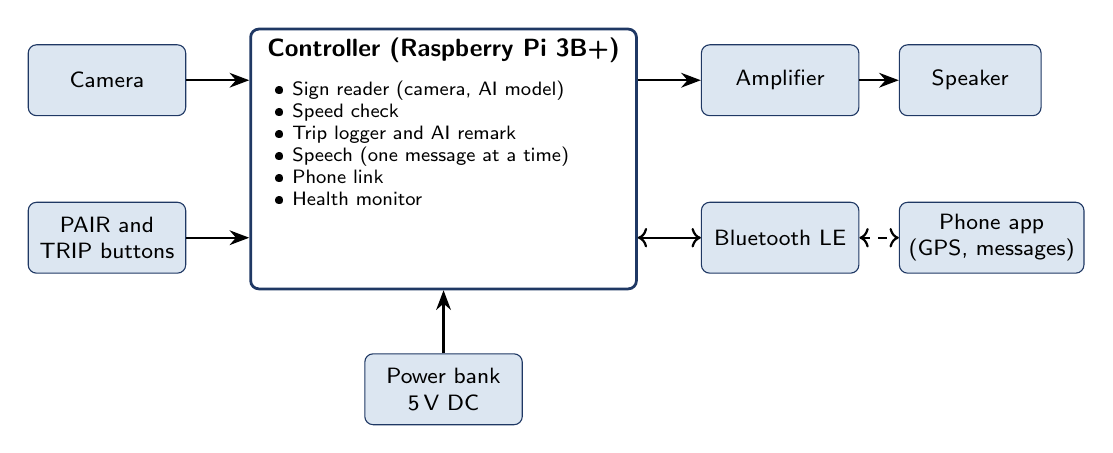
\begin{tikzpicture}[node distance=0.9cm and 1.0cm,font=\small\sffamily,
 box/.style={draw=NavyBlue,fill=LightBlue,rounded corners=3pt,minimum width=2.0cm,minimum height=0.9cm,align=center,font=\footnotesize\sffamily},
 core/.style={draw=NavyBlue,fill=white,rounded corners=3pt,minimum width=4.9cm,minimum height=3.3cm,align=center,line width=1pt},
 arr/.style={-{Stealth[length=2.5mm]},line width=0.8pt}]
 \node[core] (pi) {};
 \node[anchor=north,font=\small\sffamily\bfseries] at (pi.north) {Controller (Raspberry Pi 3B+)};
 \node[font=\scriptsize\sffamily,align=left,anchor=north west] at ($(pi.north west)+(0.2,-0.55)$) {\textbullet\ Sign reader (camera, AI model)\\ \textbullet\ Speed check\\ \textbullet\ Trip logger and AI remark\\ \textbullet\ Speech (one message at a time)\\ \textbullet\ Phone link\\ \textbullet\ Health monitor};
 \node[box,left=0.8cm of pi,yshift=1cm] (cam) {Camera};
 \node[box,left=0.8cm of pi,yshift=-1cm] (ctl) {PAIR and\\TRIP buttons};
 \node[box,right=0.8cm of pi,yshift=1cm] (amp) {Amplifier};
 \node[box,right=0.8cm of pi,yshift=-1cm] (ble) {Bluetooth LE};
 \node[box,right=0.5cm of amp,minimum width=1.8cm] (spk) {Speaker};
 \node[box,right=0.5cm of ble,minimum width=1.8cm] (app) {Phone app\\(GPS, messages)};
 \node[box,below=0.8cm of pi] (pw) {Power bank\\5\,V DC};
 \draw[arr] (cam)--(cam-|pi.west);\draw[arr] (ctl)--(ctl-|pi.west);
 \draw[arr] (amp-|pi.east)--(amp);\draw[arr] (amp)--(spk);
 \draw[arr,<->] (ble-|pi.east)--(ble);\draw[arr,<->,dashed] (ble)--(app);
 \draw[arr] (pw)--(pi);
\end{tikzpicture}
\caption{Simplified block diagram}\label{fig:block}
\end{figure}

\section{Technical Specifications}\label{sec:specs}\index{specifications}\index{power consumption}\index{running time}\index{camera!resolution}\index{Bluetooth LE!specification}\index{operating temperature}\index{IP rating}\index{dimensions}

\begin{table}[H]\centering\small
\caption{Technical specifications}
\begin{tabularx}{\linewidth}{|l|X|}\hline
\hdr{Parameter} & \hdr{Value}\\ \hline
Model & \ModelNo\\ \hline
Controller & Raspberry Pi 3B+ (quad-core 1.4\,GHz, 1\,GB RAM)\\ \hline
Power input & 5\,V DC through the unit's USB cable (USB-A plug); source of at least 2.4\,A\\ \hline
Power consumption & About 2--5\,W, depending on load (controller figures)\\ \hline
Running time on a power bank & About 6--8\,h on a 10\,000\,mAh power bank (estimate)\\ \hline
Ready after power-on & About 60\,s, confirmed by \say{Self test passed. System ready.}\\ \hline
Camera & 5\,MP camera module; signs read at 640\,$\times$\,480, 15 frames per second (10 when hot)\\ \hline
Road signs & 20 classes from IRC:67: speed limits 20, 30, 40, 50, 60, 80, 100\,km/h; stop; give way; no entry; no overtaking; no U-turn; no honking; no parking; school ahead; pedestrian crossing; speed breaker; left curve; right curve; men at work\\ \hline
Sign confirmation & Same sign seen in 3 of 5 frames; about 60\,ms processing per frame; speech starts at once\\ \hline
Overspeed warning & More than 5\,km/h over the last limit read, for 3\,s; repeated at most every 30\,s\\ \hline
Speed source & Phone GPS (fixes worse than $\pm$30\,m are ignored)\\ \hline
Audio & 3\,W, 4\,$\Omega$ speaker; class-D digital amplifier; three volume levels\\ \hline
Voice & Natural British-English female voice, generated in the unit (offline)\\ \hline
Wireless & Bluetooth Low Energy, 2.4\,GHz; pairing with a 6-digit spoken code\\ \hline
Phone app & Android 8.0 or newer\\ \hline
Trip storage & Unit: last 20 trips. App: last 200 trips. Route point about every 25\,m\\ \hline
Operating conditions & 0--45\,\textdegree C; inside the vehicle; non-condensing\\ \hline
Storage conditions & $-$10 to +60\,\textdegree C; dry\\ \hline
Ingress protection & IP20 (IEC 60529); not protected against water\\ \hline
Enclosure & General-purpose electrical junction box (PVC), cut to fit; speaker on the lid; PAIR and TRIP buttons on short leads\\ \hline
Dimensions / mass & Measured values: see the Product Test Report\\ \hline
Device software & \FWVer\ (app \AppVer)\\ \hline
\end{tabularx}\end{table}

% =====================================================================
\chapter{Installation and Setup}\label{ch:install}
\section{Before You Start}\index{installation!before you start}\index{placement!requirements}
\begin{itemize}[leftmargin=*]
\item Check the package contents (Section~\ref{sec:box}).
\item Charge the power bank fully.
\item Have ready: your Android phone, with Bluetooth and Location switched on, and an internet connection to download the app.
\item Set up the unit while the car is \textbf{parked}.
\end{itemize}
\begin{table}[H]\centering\small
\caption{Placement requirements}
\begin{tabularx}{\linewidth}{|l|X|}\hline
\hdr{Item} & \hdr{Requirement}\\ \hline
Surface & Flat part of the dashboard, near the centre of the windscreen, on a non-slip mat\\ \hline
View & Camera window \callout{1} facing straight ahead, with a clear view through the windscreen, inside the area cleared by the wipers\\ \hline
Driver's view & Below your line of sight to the road; not in front of the instruments or mirrors\\ \hline
Airbags & Not on, or in front of, any airbag cover (marked \emph{SRS} or \emph{AIRBAG})\\ \hline
Clearance & Speaker \callout{2} on the lid uncovered; at least 2\,cm free space around the case\\ \hline
Phone & Within 5\,m of the unit (inside the car), in a holder or a pocket; Bluetooth on\\ \hline
\end{tabularx}\end{table}

\section{Unpacking and Inspection}\index{unpacking}\index{inspection on delivery}
\begin{enumerate}[leftmargin=*]
\item Remove the unit and the cable from the packaging.
\item Check the case, the camera window and the cable for cracks, loose parts or bent pins.
\item Keep the packaging for transport and return (Chapter~\ref{ch:disposal}).
\end{enumerate}

\section{Placing the Unit}\label{sec:place}\index{placement}\index{dashboard placement|see{placement}}\index{windscreen}\index{non-slip mat}\index{camera!aiming}
\begin{figure}[H]\centering
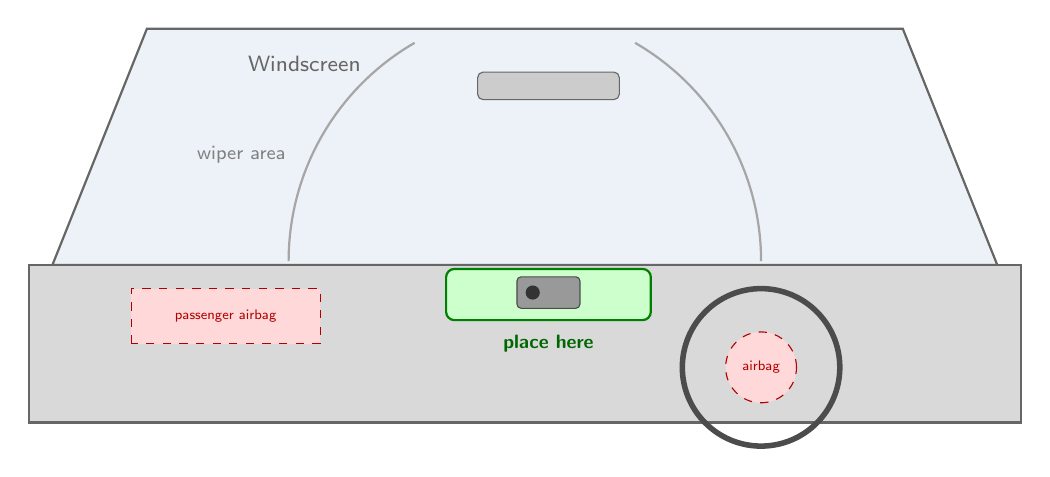
\begin{tikzpicture}[font=\footnotesize\sffamily,x=1cm,y=1cm]
 % windscreen and dashboard, seen from the driver's seat
 \draw[fill=LightBlue!50,draw=black!60,line width=0.8pt] (0,2.2)--(1.2,5.2)--(10.8,5.2)--(12,2.2)--cycle;
 \node[black!60] at (3.2,4.75) {Windscreen};
 \draw[black!35,line width=0.8pt] (3,2.25) arc(180:120:3.2);\draw[black!35,line width=0.8pt] (9,2.25) arc(0:60:3.2);
 \node[black!50,font=\scriptsize\sffamily] at (2.4,3.6) {wiper area};
 \draw[fill=black!15,draw=black!60,line width=0.8pt] (-0.3,0.2) rectangle (12.3,2.2);
 % steering wheel and airbag
 \draw[black!70,line width=2pt] (9,0.9) circle (1.0);\draw[fill=red!15,draw=red!70!black,dashed] (9,0.9) circle (0.45);
 \node[red!70!black,font=\tiny\sffamily] at (9,0.9) {airbag};
 \draw[fill=red!15,draw=red!70!black,dashed] (1.0,1.2) rectangle (3.4,1.9);\node[red!70!black,font=\tiny\sffamily] at (2.2,1.55) {passenger airbag};
 % recommended zone
 \draw[fill=green!20,draw=green!50!black,line width=0.8pt,rounded corners=3pt] (5.0,1.5) rectangle (7.6,2.15);
 \draw[fill=black!40,draw=black!70,rounded corners=1.5pt] (5.9,1.65) rectangle (6.7,2.05);\fill[black!80] (6.1,1.85) circle (0.09);
 \node[green!40!black,font=\scriptsize\sffamily\bfseries] at (6.3,1.2) {place here};
 % mirror
 \draw[fill=black!20,draw=black!60,rounded corners=2pt] (5.4,4.3) rectangle (7.2,4.65);
\end{tikzpicture}
\caption{Where to place the unit (driver's view, right-hand-drive car)}\label{fig:place}
\end{figure}
\begin{enumerate}[leftmargin=*]
\item Put a non-slip mat on the centre of the dashboard, away from the airbag covers (Figure~\ref{fig:place}).
\item Place the unit on the mat with the camera window \callout{1} facing straight ahead through the windscreen.
\item Check from the driver's seat that the unit is below your view of the road and does not reflect in the windscreen.
\item Check that the camera's view is not blocked by the rear-view mirror, a sticker or a tinted band.
\item Push gently on the unit: it must not slide. If it does, use a stronger non-slip mat.
\item Lay the \ui{PAIR} and \ui{TRIP} buttons where you can reach them while parked, clear of the pedals, the gear lever and the steering wheel.
\end{enumerate}
\begin{tip}
The camera reads signs best when it is level and looks slightly to the left of the lane, where Indian road signs stand. A clean windscreen makes a large difference at night and in the rain.
\end{tip}

\section{Connecting Power}\label{sec:power}\index{power bank!connecting}\index{car USB charger}\index{power source!car charger}\index{ended with a power cut}
\begin{figure}[H]\centering
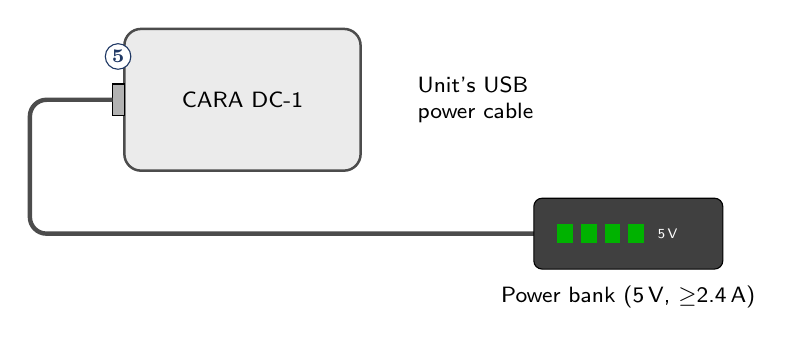
\begin{tikzpicture}[font=\footnotesize\sffamily]
 \draw[fill=black!8,draw=black!70,line width=0.9pt,rounded corners=6pt] (0,0) rectangle (3,1.8);\node at (1.5,0.9) {\Brand\ \ModelNo};
 \draw[fill=black!30] (-0.15,0.7) rectangle (0,1.1);
 \node[circle,draw=NavyBlue,fill=white,inner sep=1pt,text=NavyBlue,font=\bfseries\scriptsize] at (-0.08,1.45) {5};
 \draw[line width=1.6pt,black!70,rounded corners=6pt] (-0.15,0.9)--(-1.2,0.9)--(-1.2,-0.8)--(5.2,-0.8);
 \draw[fill=black!75,rounded corners=3pt] (5.2,-1.25) rectangle (7.6,-0.35);
 \foreach \x in {5.5,5.8,6.1,6.4}{\fill[green!70!black] (\x,-0.92) rectangle (\x+0.2,-0.68);}
 \node[white,font=\tiny\sffamily] at (6.9,-0.8) {5\,V};
 \node at (6.4,-1.6) {Power bank (5\,V, $\ge$2.4\,A)};
 \node[align=left,anchor=west] at (3.6,0.9) {Unit's USB\\power cable};
\end{tikzpicture}
\caption{Connecting the power bank}\label{fig:power}
\end{figure}
\subsection*{Standard: power bank}
\begin{enumerate}[leftmargin=*]
\item Plug the unit's USB power cable \callout{5} into the power bank. The unit switches on.
\item Wait about 60\,s. The unit speaks \spk\ \say{Self test passed. System ready.}
\item Put the power bank where it cannot slide (for example in the door pocket or the centre console), out of direct sunlight.
\end{enumerate}

\subsection*{Option: car USB charger}
You can power the unit from a USB charger in the car's 12\,V socket, if the charger gives \textbf{5\,V and at least 2.5\,A} on one port.
\begin{notice}
In most cars the 12\,V socket switches off with the key. The unit then loses power at the moment you park, before it can speak the trip summary and send the trip to the app. The trip is closed later and marked \emph{ended with a power cut}. Use a power bank if you want the summary every time. A weak charger makes the unit slow down; if the unit often restarts or alerts come late, change to a stronger charger or a power bank.
\end{notice}

\section{Installing the App}\label{sec:app}\index{app!installing}\index{APK}\index{Play Protect}
\begin{enumerate}[leftmargin=*]
\item On the phone, open the app link from the Quick Start Guide or from \field{\Website}{website} and download the \AppName\ app (file \texttt{.apk}).
\item Open the downloaded file. If Android asks, allow installing apps from this source.
\item If \emph{Play Protect} shows a warning, tap \ui{More details}, then \ui{Install anyway}. (The prototype app is not yet in the Play Store.)
\item Open the \AppName\ app.
\end{enumerate}

\subsection*{Allowing the permissions}\index{permissions}\index{Notification access}\index{Location!permission}\index{restricted setting}\index{battery saver}
Under \ui{Permissions needed}, tap \ui{Allow} for each line until the panel shows \ui{All permissions allowed}.
\begin{table}[H]\centering\small
\caption{App permissions}
\begin{tabularx}{\linewidth}{|l|X|}\hline
\hdr{Permission} & \hdr{Why it is needed}\\ \hline
Bluetooth & To find and connect to the unit\\ \hline
Notification access & To announce messages, text messages and calls. Android opens a settings page: switch on \emph{\AppName}\\ \hline
Location (precise) & To send the car's speed and the route of each trip to the unit\\ \hline
Notifications & To show the connection status while the app runs in the background\\ \hline
\end{tabularx}\end{table}
\begin{tip}
If Android says \emph{Restricted setting} for Notification access: open \menu{Settings $\rightarrow$ Apps $\rightarrow$ \AppName}, tap the \menu{\vdots} menu, choose \ui{Allow restricted settings}, and try again. To keep the connection when the phone sleeps, set \menu{Settings $\rightarrow$ Apps $\rightarrow$ \AppName\ $\rightarrow$ Battery} to \ui{Unrestricted}.
\end{tip}

\section{Pairing the Phone (First Time)}\label{sec:pair}\index{pairing}\index{pairing code}\index{Pairing mode on}\index{Phone paired}
\begin{enumerate}[leftmargin=*]
\item Check that the unit is on and has said \say{System ready.}
\item Press and hold the \ui{PAIR} button \callout{3} for 5\,s, until the unit says \spk\ \say{Pairing mode on.} Release the button.
\item Within 2 minutes, tap \ui{Pair} in the app.
\item Android shows a pairing box. Type the 6-digit code that the unit speaks, and tap \ui{Pair}.
\item The unit says \spk\ \say{Phone paired.} The app shows \sdot{green!60!black}\ \ui{Connected}.
\end{enumerate}
\begin{notice}
Pairing mode closes by itself after 2 minutes (\say{Pairing mode off.}). Only a phone that typed the spoken code can connect. Do not pair while someone outside the car can hear the code.
\end{notice}

\section{First-Time Check}\label{sec:firsttime}\index{first-time check}\index{Send test alert}\index{test alert|see{Send test alert}}
\begin{enumerate}[leftmargin=*]
\item In the app, tap \ui{Send test alert}. The unit says a test message.
\item Under \ui{Announcements}, set the \ui{Volume} (Section~\ref{sec:settings}) and tap \ui{Send test alert} again until the level suits you.
\item Ask someone to send you a WhatsApp message or a text message. The unit announces it.
\item Check that the \ui{Phone GPS} line on the home screen turns green (this needs an outdoor view of the sky).
\end{enumerate}
After the first pairing, the app connects again by itself whenever the unit is on and the phone is in range.

% =====================================================================
\chapter{Operation}\label{ch:operation}
\section{Switching On and Off}\index{switching on}\index{switching off}\index{restart}\index{power cut}
\begin{table}[H]\centering\small
\caption{Power control}
\begin{tabularx}{\linewidth}{|l|X|}\hline
\hdr{Action} & \hdr{How}\\ \hline
Switch on & Plug the power cable \callout{5} into the power source. Ready in about 60\,s: \say{Self test passed. System ready.}\\ \hline
Switch off & Press \ui{TRIP} \callout{4} to end the trip, wait until the trip summary has been spoken and the trip appears in the app, then unplug the power cable\\ \hline
Restart & Disconnect the power, wait 10\,s, connect it again (use only if the unit does not respond)\\ \hline
\end{tabularx}\end{table}
\begin{notice}
The unit is designed to survive a sudden loss of power without damage to its data. A power cut during a drive can lose up to the last minute of that trip.
\end{notice}

\section{What the Unit Says}\label{sec:voice}\index{voice messages}\index{spoken messages|see{voice messages}}\index{Self test passed}\index{self-test}\index{Sign alerts paused}\index{connection status}\index{status dot|see{connection status}}
The unit has no screen and no lights: it tells you its state by voice. The app's status dot shows the connection.
\begin{table}[H]\centering\small
\caption{Status and system messages}\label{tab:voice}
\begin{tabularx}{\linewidth}{|>{\raggedright\arraybackslash}p{0.38\linewidth}|X|}\hline
\hdr{The unit says} & \hdr{Meaning / action}\\ \hline
\spk\ \say{Self test passed. System ready.} & Started correctly; ready to drive\\ \hline
\spk\ \say{Self test: \ldots} & Started, but something is wrong (it names the part). See Table~\ref{tab:errors}\\ \hline
\spk\ \say{Pairing mode on.} / \say{Pairing mode off.} & A new phone can pair for 2 minutes / pairing closed\\ \hline
\spk\ \say{Phone paired.} & A phone has paired successfully\\ \hline
\spk\ \say{Trip started.} / \say{Trip ended.} & You pressed \ui{TRIP}; a trip has started / ended\\ \hline
\spk\ \say{Sign alerts paused.} & The camera has been blocked, dark or dazzled for 10\,s. Overspeed warnings continue\\ \hline
\spk\ \say{Sign alerts resumed.} & The camera can see again\\ \hline
\spk\ \say{Camera not found. Sign alerts are off.} & The camera is not working. See Table~\ref{tab:errors}\\ \hline
\spk\ \say{Warning: the \ldots\ stopped working.} & One part of the software stopped; it restarts itself within seconds\\ \hline
\end{tabularx}\end{table}
\begin{table}[H]\centering\small
\caption{Connection status in the app}
\begin{tabularx}{\linewidth}{|c|l|X|}\hline
\hdr{Dot} & \hdr{Text} & \hdr{Meaning}\\ \hline
\sdot{green!60!black} & \ui{Connected} & Phone and unit are linked\\ \hline
\sdot{Amber} & \ui{Searching\ldots}, \ui{Connecting\ldots} & The app is looking for the unit\\ \hline
\sdot{red!75!black} & \ui{Bluetooth is off}, \ui{Disconnected} & Switch on Bluetooth, or bring the phone near the unit\\ \hline
\sdot{black!40} & \ui{Not connected} & Not paired yet, or you tapped \ui{Disconnect}\\ \hline
\end{tabularx}\end{table}

\section{A Normal Drive}\label{sec:normal}\index{drive, normal}\index{trip!starting}\index{trip!ending}\index{short trips}
\begin{enumerate}[leftmargin=*]
\item Connect the power and wait for \say{System ready.} The app connects by itself.
\item Check that the app shows \ui{Connected} and a green \ui{Phone GPS} line. Put the phone away.
\item Press the \ui{TRIP} button \callout{4} once, before you set off. The unit says \spk\ \say{Trip started.}
\item Drive. The unit speaks road signs, overspeed warnings and your chosen announcements.
\item When you have parked, press \ui{TRIP} again. The unit says \spk\ \say{Trip ended.} and then speaks the trip summary.
\item Look at the trip in the app later (Section~\ref{sec:trips}).
\end{enumerate}
\begin{figure}[H]\centering
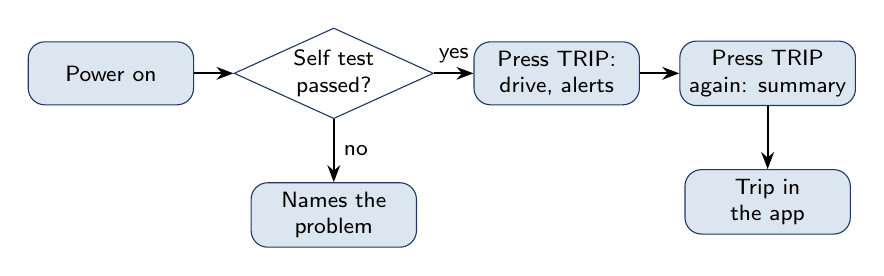
\begin{tikzpicture}[node distance=0.5cm,font=\footnotesize\sffamily,
 st/.style={draw=NavyBlue,fill=LightBlue,rounded corners=6pt,minimum width=2.1cm,minimum height=0.8cm,align=center},
 dc/.style={draw=NavyBlue,fill=white,diamond,aspect=2.2,inner sep=1pt,align=center},
 ar/.style={-{Stealth},line width=0.7pt}]
 \node[st] (s1) {Power on};
 \node[dc,right=of s1] (d) {Self test\\passed?};
 \node[st,right=of d] (s2) {Press TRIP:\\drive, alerts};
 \node[st,right=of s2] (s3) {Press TRIP\\again: summary};
 \node[st,below=0.8cm of d] (e) {Names the\\problem};
 \node[st,below=0.8cm of s3] (s4) {Trip in\\the app};
 \draw[ar] (s1)--(d);\draw[ar] (d)--node[above]{yes}(s2);\draw[ar] (s2)--(s3);\draw[ar] (s3)--(s4);\draw[ar] (d)--node[right]{no}(e);
\end{tikzpicture}
\caption{Start-up and drive sequence}
\end{figure}
\begin{tip}
Trips shorter than 100\,m are not kept (for example when you only move the car in the driveway). Waiting in traffic does not end a trip: only the \ui{TRIP} button does.
\end{tip}

\section{Road-Sign Alerts}\label{sec:signs}\index{road signs}\index{sign list}\index{speed limit signs}\index{road signs!limitations}
While a trip is running, the camera looks for the 20 signs listed in Table~\ref{tab:signs}. When it has seen the same sign in 3 of 5 pictures, it speaks it once. A sign is spoken again only when it is seen again later.
\begin{table}[H]\centering\small
\caption{Road signs and what the unit says}\label{tab:signs}
\begin{tabularx}{\linewidth}{|l|X||l|X|}\hline
\hdr{Sign} & \hdr{The unit says} & \hdr{Sign} & \hdr{The unit says}\\ \hline
Speed limit 20--100 & \say{Speed limit 50.} (the number read) & No parking & \say{No parking.}\\ \hline
Stop & \say{Stop sign ahead.} & School ahead & \say{School ahead.}\\ \hline
Give way & \say{Give way.} & Pedestrian crossing & \say{Pedestrian crossing ahead.}\\ \hline
No entry & \say{No entry.} & Speed breaker & \say{Speed breaker ahead.}\\ \hline
No overtaking & \say{No overtaking.} & Left curve & \say{Left curve ahead.}\\ \hline
No U-turn & \say{No U-turn.} & Right curve & \say{Right curve ahead.}\\ \hline
No honking & \say{No honking.} & Men at work & \say{Men at work ahead.}\\ \hline
\end{tabularx}\end{table}
\begin{warning}
Signs can be missed or misread when they are dirty, damaged, bent, hidden by trees or vehicles, very far away, or at night, in rain, fog or strong glare. Other signs are not recognised. Always look at the signs yourself.
\end{warning}

\section{Overspeed Warnings}\label{sec:overspeed}\index{overspeed}\index{speed limit!forgetting}\index{Slow down warning}
The unit compares the car's speed (from the phone's GPS) with the \textbf{last speed-limit sign it read}.
\begin{itemize}[leftmargin=*]
\item When you are more than \textbf{5\,km/h over} that limit for \textbf{3\,s}, it says \spk\ \say{Slow down. Speed limit 50.} This warning is spoken before anything else.
\item While you stay over the limit, the warning is repeated at most every 30\,s.
\item The warning ends when you have been back under the limit for 2\,s.
\item The limit is forgotten after \textbf{5\,km}, or when the trip ends, so an old sign never causes a warning later.
\end{itemize}
\begin{notice}
No warning is given when no speed-limit sign has been read in the last 5\,km, or when the phone's GPS is weak (worse than $\pm$30\,m, for example in tunnels or under flyovers). The phone's speed can lag by a second or two.
\end{notice}

\section{Phone Announcements}\label{sec:announce}\index{announcements}\index{WhatsApp}\index{text messages (SMS)}\index{calls, incoming}\index{priority of alerts}
When the phone is connected, the unit announces:
\begin{table}[H]\centering\small
\caption{Announcements}
\begin{tabularx}{\linewidth}{|l|X|}\hline
\hdr{Event} & \hdr{The unit says (example)}\\ \hline
Message from a chosen app & \say{WhatsApp message from Rahul.} With \ui{Read message text} on: followed by the message\\ \hline
Text message (SMS) & \say{Text message from Mum.}\\ \hline
Incoming call & \say{Incoming call from Priya.}\\ \hline
\end{tabularx}\end{table}
The unit speaks one thing at a time, most urgent first: overspeed warnings, then road signs, then calls, then messages, then system messages. An announcement that has waited too long is dropped, so you never hear an old call. \ui{Quiet mode} stops all phone announcements; road alerts continue.

\section{Trip Summary and Trip History}\label{sec:trips}\index{trip summary}\index{AI remark}\index{trip history}\index{map!route}\index{route|see{map}}
When you press \ui{TRIP} to end the trip, the unit says \say{Trip ended.} and then speaks:
\begin{enumerate}[leftmargin=*]
\item a sentence with the facts of the drive (distance, time, warnings), at once; then
\item one short remark written by the on-device AI, after about 5--8\,s. The very first remark after the unit is switched on can take up to a minute.
\end{enumerate}
The numbers always come from the trip log, never from the AI. If the AI's remark does not pass the unit's checks, only the facts are spoken.

In the app, the trip appears under \ui{Recent trips}; tap it to see:
\begin{itemize}[leftmargin=*]
\item the route on a map (drag and pinch to move; the map needs mobile data, the route line does not);
\item the distance, trip time and top speed, the average speed, driving time and stops;
\item the summary;
\item the details: overspeed warnings, time over the limit, road signs read and stops. \ui{Harsh braking} and \ui{Harsh acceleration} show \ui{Not measured yet} on this model.
\end{itemize}
The unit keeps the last 20 trips and sends each one until the app confirms it, so a trip is not lost when the phone was away. The app keeps the last 200 trips.

\section{Phone GPS}\index{GPS}\index{Phone GPS line}\index{speed source}
While connected, the app sends the phone's location and speed to the unit once a second. The \ui{Phone GPS} line on the home screen shows what is sent: green with the accuracy and speed, or amber when there is no fix yet or the fix is too weak. Keep Location on, with \emph{precise location} allowed.

\section{Settings Reference}\label{sec:settings}\index{settings}\index{volume}\index{Read message text}\index{Quiet mode}\index{apps to announce}
All settings are in the app under \ui{Announcements}. The unit receives each change at once and keeps it.
\begin{table}[H]\centering\small
\caption{User-adjustable settings}
\begin{tabularx}{\linewidth}{|>{\raggedright\arraybackslash}p{2.7cm}|>{\raggedright\arraybackslash}p{3.3cm}|>{\raggedright\arraybackslash}p{2.3cm}|X|}\hline
\hdr{Setting} & \hdr{Options} & \hdr{Default} & \hdr{Description}\\ \hline
\ui{Volume} & Low, Medium, High & Medium & Loudness of everything the unit says\\ \hline
\ui{Read message text} & On, Off & Off & Off: only the app and the sender are spoken\\ \hline
\ui{Quiet mode} & On, Off & Off & Road alerts only; no messages or calls\\ \hline
\ui{Incoming calls} & On, Off & On & Announce who is calling\\ \hline
\ui{SMS} & On, Off & On & Announce text messages from the default messages app\\ \hline
\ui{Apps to announce} & WhatsApp, WhatsApp Business, Telegram, Instagram, Messenger, Signal, Gmail & WhatsApp, WhatsApp Business & Tap an app to switch it on (amber dot) or off\\ \hline
\end{tabularx}\end{table}

% =====================================================================
\chapter{Maintenance}\label{ch:maint}
\begin{caution}
Disconnect the power before cleaning or any maintenance work.
\end{caution}
\section{Maintenance Schedule}\index{maintenance!schedule}
\begin{table}[H]\centering\small
\caption{Preventive maintenance schedule}
\begin{tabularx}{\linewidth}{|l|X|l|c|}\hline
\hdr{Interval} & \hdr{Task} & \hdr{Section} & \hdr{Who}\\ \hline
Before each drive & Check the cable, the case and the camera window; listen for \say{System ready.} & --- & User\\ \hline
Weekly & Clean the camera window and the windscreen in front of it & \ref{sec:cleaning} & User\\ \hline
Monthly & Clean the case and the speaker; check that the unit does not slide & \ref{sec:cleaning} & User\\ \hline
When announced & Install the new app version or device software & \ref{sec:fw} & User / Tech.\\ \hline
\end{tabularx}\end{table}

\section{Cleaning}\label{sec:cleaning}\index{cleaning}\index{camera window!cleaning}
\begin{enumerate}[leftmargin=*]
\item Wipe the camera window \callout{1} with a dry microfibre cloth, such as a spectacle cloth.
\item Wipe the case with a soft, slightly damp, lint-free cloth. Dry it at once.
\item Dust the speaker \callout{2} gently with a soft, dry brush. Do not press on the speaker cone.
\end{enumerate}
\begin{notice}
Do not use solvents, glass cleaner, abrasive cleaners or sprays on the unit, and do not let liquid enter the case through the camera window or the cable openings.
\end{notice}

\section{Heat}\index{heat!slower alerts}\index{throttling|see{heat}}
On hot days the unit slows its camera to protect itself, and sign alerts may come slightly later. Keep the unit uncovered and out of direct sun where possible, and do not leave the unit in a parked car in the sun.

\section{Software Updates}\label{sec:fw}\index{software update}\index{app!updating}\index{device software!updating}
\subsection*{App}
Download the new version from the same link (Section~\ref{sec:app}) and install it over the old one. Your trips, settings and pairing are kept.
\subsection*{Device software (Technician only)}
The device software is updated with a laptop, by a technician. Settings, trips, the phone pairing and the voice are kept.
\begin{enumerate}[leftmargin=*]
\item Connect a laptop to the unit through the service connection described in the service notes.
\item Copy the new software to the unit and run the installer (\texttt{sudo bash install.sh}).
\item Restart the unit if the installer asks.
\item Check that the unit says \say{Self test passed. System ready.} and that the app shows the new software version under the device name.
\end{enumerate}
\begin{notice}Do not disconnect the power during an update. If an update stops, run the installer again.\end{notice}

\section{Storage and Transport}\index{storage}\index{transport}
Store the unit in its packaging at $-$10 to +60\,\textdegree C, in a dry place. Disconnect the power bank and store it separately, about half charged.

\section{Spare Parts and Service}\index{spare parts}\index{service}
\begin{table}[H]\centering\small
\caption{Replaceable parts}
\begin{tabularx}{\linewidth}{|l|X|l|}\hline
\hdr{Part} & \hdr{Description / specification} & \hdr{Who replaces it}\\ \hline
Power cable & USB-A to micro-USB, rated 2.4\,A or more; routed into the case & Technician\\ \hline
PAIR and TRIP buttons & Momentary push buttons on leads with 2.54\,mm sockets & Technician\\ \hline
Camera module & Raspberry Pi camera, 5\,MP, ribbon cable & Technician\\ \hline
Speaker & 3\,W, 4\,$\Omega$, 3-inch & Technician\\ \hline
Amplifier & MAX98357A I2S class-D amplifier board & Technician\\ \hline
microSD card & Card with the device software & Technician\\ \hline
\end{tabularx}\end{table}
\begin{figure}[H]\centering
\photo{inside_labeled.jpg}{0.86\linewidth}{9cm}{Inside the unit}
\caption{Inside the unit, lid removed (Technician only)}\label{fig:inside}
\end{figure}
Every module plugs in; no soldering is needed to replace it (Figure~\ref{fig:inside}). Service must be carried out only by the \Brand\ team or a trained technician. Contact: \field{\SupportMail}{e-mail}.

% =====================================================================
\chapter{Troubleshooting}\label{ch:trouble}
\section{Quick Diagnosis Flow}\index{troubleshooting!unit does not start}
\begin{figure}[H]\centering
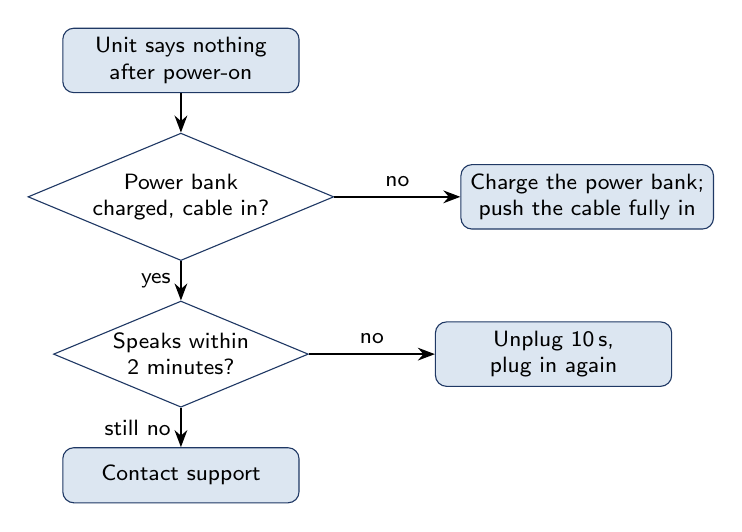
\begin{tikzpicture}[node distance=0.5cm,font=\footnotesize\sffamily,
 st/.style={draw=NavyBlue,fill=LightBlue,rounded corners=4pt,minimum width=3cm,minimum height=0.7cm,align=center},
 dc/.style={draw=NavyBlue,fill=white,diamond,aspect=2.4,inner sep=1pt,align=center},
 ar/.style={-{Stealth},line width=0.7pt}]
 \node[st] (a) {Unit says nothing\\after power-on};
 \node[dc,below=of a] (b) {Power bank\\charged, cable in?};
 \node[st,right=1.6cm of b] (c) {Charge the power bank;\\push the cable fully in};
 \node[dc,below=of b] (d) {Speaks within\\2 minutes?};
 \node[st,right=1.6cm of d] (e) {Unplug 10\,s,\\plug in again};
 \node[st,below=of d] (f) {Contact support};
 \draw[ar] (a)--(b);\draw[ar] (b)--node[above]{no}(c);\draw[ar] (b)--node[left]{yes}(d);
 \draw[ar] (d)--node[above]{no}(e);\draw[ar] (d)--node[left]{still no}(f);
\end{tikzpicture}
\caption{Troubleshooting flow: the unit does not start}
\end{figure}

\section{Symptoms, Causes and Remedies}\index{troubleshooting}\index{app does not find the unit}\index{no road-sign alerts}\index{no overspeed warnings}\index{no trip summary}\index{map is blank}
\begin{table}[H]\centering\small
\caption{Troubleshooting table}
\begin{tabularx}{\linewidth}{|p{0.24\linewidth}|X|X|}\hline
\hdr{Symptom} & \hdr{Possible cause} & \hdr{Remedy}\\ \hline
The app does not find the unit & Pairing mode not on; Bluetooth off; old pairing on the phone & Hold \ui{PAIR} 5\,s again; switch on Bluetooth (and Location on Android 11 or older); remove any old \emph{DC-\ldots} entry in Android's Bluetooth settings and pair again\\ \hline
Pairing box does not appear, or \ui{Pairing failed} & Pairing mode closed after 2 minutes; wrong code & Hold \ui{PAIR} again and type the code at once\\ \hline
Connected, but messages are not announced & Notification access off; app not chosen; Quiet mode on & Allow Notification access; switch the app on under \ui{Apps to announce}; switch Quiet mode off\\ \hline
Connection drops when the phone sleeps & Battery saver stops the app & Set the app's battery use to \ui{Unrestricted}\\ \hline
No road-sign alerts & No trip running; camera blocked; \say{Sign alerts paused.} & Press \ui{TRIP} (it says \say{Trip started.}); clean the camera window and the windscreen; point the unit forward\\ \hline
No overspeed warnings & No speed-limit sign read; weak phone GPS & Normal behaviour without a sign; check the \ui{Phone GPS} line is green\\ \hline
Alerts come late or the unit restarts & Weak power source; unit too hot & Use a power bank of 2.4\,A or more; keep the unit uncovered and out of the sun\\ \hline
No trip summary when parking & Power lost with the key (car charger) & Use a power bank (Section~\ref{sec:power})\\ \hline
Map is blank but the route shows & No mobile data on the phone & The map needs data; the route is stored anyway\\ \hline
The voice is too quiet or too loud & Volume setting & Change \ui{Volume} in the app\\ \hline
\end{tabularx}\end{table}

\section{Spoken Warnings}\index{spoken warnings}\index{error codes|see{spoken warnings}}\index{Camera not found}
The unit has no error codes. It names the problem instead.
\begin{table}[H]\centering\small
\caption{Spoken warnings}\label{tab:errors}
\begin{tabularx}{\linewidth}{|>{\raggedright\arraybackslash}p{0.36\linewidth}|l|X|}\hline
\hdr{The unit says} & \hdr{Meaning} & \hdr{Action}\\ \hline
\say{Self test: \ldots} & A part failed at start & Restart the unit; if repeated, contact support\\ \hline
\say{Camera not found. Sign alerts are off.} & Camera not detected & Restart; if repeated, contact support. Overspeed and announcements still work\\ \hline
\say{The sign reader could not start.} & Sign software fault & Restart; if repeated, contact support\\ \hline
\say{Sign alerts paused.} & Camera blocked or dazzled for 10\,s & Clean the window; it resumes by itself\\ \hline
\say{Warning: the speech stopped working.} (or another part) & One software part stopped & It restarts by itself; if repeated, restart the unit\\ \hline
\end{tabularx}\end{table}

\section{Removing a Pairing}\index{pairing!removing}\index{new phone, connecting}
To connect a different phone, or after a pairing problem:
\begin{enumerate}[leftmargin=*]
\item On the old phone, open \menu{Settings $\rightarrow$ Bluetooth} and remove (\ui{Forget}) the \emph{DC-\ldots} device.
\item Pair the new phone as in Section~\ref{sec:pair}.
\end{enumerate}

\section{When to Contact Support}\index{support!when to contact}
Contact support if the problem continues after the remedies above, if the case is damaged, or if you notice smoke, a burning smell or a swollen power bank (stop using it at once). Have ready: the model, the device software version (shown under the device name in the app), the app version, what the unit said, and a short description.

% =====================================================================
\chapter{Disposal and Environment}\label{ch:disposal}

\section{Do Not Dispose of with Household Waste}\index{disposal}\index{e-waste}
\begin{center}\weeesym[1.2cm]\end{center}
This symbol means the product must \textbf{not} be put in household waste. Electrical and electronic equipment contains materials that can harm the environment and health if handled incorrectly, and valuable materials that can be recovered.

\section{How to Dispose of the Product}\index{disposal!steps}\index{data!erasing}
\begin{enumerate}[leftmargin=*]
\item \textbf{Remove your data.} Ask a technician to erase the trips stored in the unit, or remove its microSD card. In the app, uninstall the \AppName\ app to delete the trips on the phone, and remove the \emph{DC-\ldots} pairing in Android's Bluetooth settings.
\item \textbf{Separate the power bank.} The unit has no internal battery. Dispose of the power bank separately at a battery collection point.
\item \textbf{Hand over} the unit and the cable to an authorised e-waste collection point or recycler: \field{\Website}{take-back details on the website}.
\item Keep the receipt or recycling certificate, if one is issued.
\end{enumerate}

\section{Applicable Regulations}\index{regulations}\index{E-Waste Rules}
\begin{table}[H]\centering\small
\caption{Regulations on end-of-life handling (check the current edition and your local rules)}
\begin{tabularx}{\linewidth}{|l|X|}\hline
\hdr{Regulation} & \hdr{Relevance}\\ \hline
E-Waste (Management) Rules, 2022, India & Producer responsibility, collection and authorised recycling of electronic waste\\ \hline
Battery Waste Management Rules, 2022, India & Collection and recycling of used batteries (the power bank)\\ \hline
WEEE Directive 2012/19/EU & Separate collection and recovery of electrical and electronic equipment (EU)\\ \hline
RoHS Directive 2011/65/EU & Restriction of hazardous substances in the product\\ \hline
\end{tabularx}\end{table}

\section{Material Information}\index{materials}\index{recycling}
\begin{table}[H]\centering\small
\caption{Main materials (to help recyclers)}
\begin{tabularx}{\linewidth}{|l|X|l|}\hline
\hdr{Component} & \hdr{Material} & \hdr{Recycling route}\\ \hline
Case & General-purpose electrical junction box, PVC plastic & Plastics\\ \hline
Buttons & Plastic push buttons, copper leads & E-waste\\ \hline
Circuit boards (controller, amplifier, camera) & FR-4 laminate, copper, solder & E-waste\\ \hline
Speaker & Steel, magnet, paper cone & E-waste\\ \hline
Cable & Copper, PVC & E-waste\\ \hline
Packaging & Cardboard, paper & Paper recycling\\ \hline
\end{tabularx}\end{table}

\section{Packaging}
Recycle the packaging according to local rules. Cardboard and paper go to paper recycling.

% =====================================================================
\chapter{Warranty, Support and Compliance}\label{ch:compliance}
\section{Warranty}\index{warranty}
The \ModelNo\ is an educational prototype and is supplied without a commercial warranty. Report any fault to the \Brand\ team (see Technical Support below). Damage from misuse, opening the case, liquids, drops, heat, or power sources other than those in Section~\ref{sec:power} is not covered.

\section{Technical Support}\index{support!contact}\index{e-mail, support|see{support}}
\begin{table}[H]\centering\small
\begin{tabularx}{\linewidth}{|l|X|}\hline
\hdr{Contact} & \hdr{Details}\\ \hline
E-mail & \field{\SupportMail}{e-mail}\\ \hline
Website / downloads & \field{\Website}{website}\\ \hline
Address & \TeamName, \DeptName, \InstituteName, Bhubaneswar, Odisha, India\\ \hline
\end{tabularx}\end{table}

\section{Regulatory Compliance}\index{compliance}\index{certification|see{compliance}}
\begin{table}[H]\centering\small
\caption{Compliance information}
\begin{tabularx}{\linewidth}{|l|X|l|}\hline
\hdr{Area} & \hdr{Standard / regulation} & \hdr{Status}\\ \hline
Product safety & IEC 62368-1 (instructional safeguards applied in this manual) & Not tested\\ \hline
EMC & CISPR 32; IEC 61000-4-2 & Not tested\\ \hline
Radio & Bluetooth LE radio of the Raspberry Pi 3B+ board & Board manufacturer's own conformity\\ \hline
Hazardous substances & RoHS & Not assessed\\ \hline
Instructions for use & IEC/IEEE 82079-1 & This manual\\ \hline
\end{tabularx}\end{table}
\begin{notice}
This product is an educational prototype and has not been certified for commercial sale.
\end{notice}

\section{Declaration of Conformity}
Not applicable: no declaration of conformity has been issued for this prototype.

% =====================================================================
\appendix
\chapter{Quick Reference Card}\index{quick reference}
\begin{table}[H]\centering\small
\begin{tabularx}{\linewidth}{|l|X|}\hline
\hdr{Task} & \hdr{Action}\\ \hline
Switch on & Connect the power; wait for \say{System ready.}\\ \hline
Start a trip & Press \ui{TRIP} \callout{4} (\say{Trip started.})\\ \hline
End a trip and hear the summary & Press \ui{TRIP} again (\say{Trip ended.})\\ \hline
Switch off & After the summary, unplug the power cable\\ \hline
Pair a new phone & Hold \ui{PAIR} \callout{3} for 5\,s, then \ui{Pair} in the app and type the spoken code\\ \hline
Test the speaker & App: \ui{Send test alert}\\ \hline
Road alerts only & App: \ui{Quiet mode} on\\ \hline
Restart & Disconnect the power for 10\,s\\ \hline
Support & \field{\SupportMail}{e-mail}\\ \hline
\end{tabularx}\end{table}

\chapter{Connector and Interface Details}\index{connector pins}\index{GPIO pins|see{connector pins}}
\begin{table}[H]\centering\small
\caption{Internal connections (Technician only); pin numbers on the controller's 40-pin header}
\begin{tabularx}{\linewidth}{|l|l|l|X|}\hline
\hdr{Part} & \hdr{Pin} & \hdr{Signal} & \hdr{Description}\\ \hline
\ui{PAIR} button & 11 / 9 & GPIO17 / GND & Pressed = low; held 5\,s = pairing mode\\ \hline
\ui{TRIP} button & 13 / 14 & GPIO27 / GND & Pressed = low; each press starts or ends a trip\\ \hline
Amplifier & 2 / 6 & 5\,V / GND & Supply\\ \hline
 & 12 / 35 / 40 & BCLK / LRC / DIN & Digital audio (I2S)\\ \hline
 & 39 & GAIN to GND & Fixed gain (12\,dB)\\ \hline
Speaker & --- & + / $-$ & On the amplifier's screw terminals only; never to GND\\ \hline
Camera & CSI & Ribbon & Camera connector, blue side towards the audio jack\\ \hline
Power & micro-USB & 5\,V DC & Controller power input\\ \hline
\end{tabularx}\end{table}

\chapter{Glossary}\index{glossary}
\begin{tabular}{lp{0.75\linewidth}}
\textbf{AI remark} & The one-sentence comment at the end of the trip summary, written by a small language model running inside the unit\\
\textbf{Bluetooth LE} & Bluetooth Low Energy, the short-range radio link between the phone and the unit\\
\textbf{GPS fix} & A position and speed measured by the phone's satellite receiver\\
\textbf{IRC:67} & The Indian Roads Congress code for road signs\\
\textbf{Overspeed} & Driving more than 5\,km/h above the last speed limit read\\
\textbf{Pairing} & Making a trusted Bluetooth link between the phone and the unit, once\\
\textbf{Quiet mode} & An app setting that keeps road alerts and stops phone announcements\\
\textbf{Trip} & One drive, from one press of \ui{TRIP} to the next\\
\textbf{WEEE} & Waste electrical and electronic equipment\\
\textbf{IP code} & Ingress protection rating (IEC 60529)\\
\end{tabular}

\clearpage\phantomsection\addcontentsline{toc}{chapter}{Index}
\printindex
\end{document}
